% Interesting trick to instead make the chapter number the letter A for this appendix.
\begingroup
\renewcommand\thechapter{A}
\titleformat{\chapter}[display]
{\normalfont\huge\bfseries}{}{20pt}{\Huge}
\setcounter{section}{0} % Set the section counter back to 0 so Chapter 4 doesn't interfere.
\setcounter{figure}{0} % Set the figure counter back to 0 so Chapter 4 doesn't interfere.

\chapter*{Appendix A - Software Installation}
\addcontentsline{toc}{chapter}{Appendix A - Software Installation}
\markboth{Appendix A}{}

\section{Miniconda}

\begin{figure}[H]
    \centering
    \includegraphics[width=.75\linewidth]{Implementation/Conda/Installation/1.png}
    \caption{Getting the latest Miniconda installation script.}
    \label{fig:CondaInstall1}
\end{figure}

\begin{figure}[H]
    \centering
    \includegraphics[width=.75\linewidth]{Implementation/Conda/Installation/2.png}
    \caption{Executing the Miniconda installation script.}
    \label{fig:CondaInstall2}
\end{figure}

% \begin{figure}[H]
%     \centering
%     \includegraphics[width=.75\linewidth]{Implementation/Conda/Installation/3.png}
%     \caption{Agreeing to Miniconda's license terms.}
%     \label{fig:CondaInstall3}
% \end{figure}

\begin{figure}[H]
    \centering
    \includegraphics[width=.75\linewidth]{Implementation/Conda/Installation/4.png}
    \caption{Making Conda run automatically in all shells.}
    \label{fig:CondaInstall4}
\end{figure}

\begin{figure}[H]
    \centering
    \includegraphics[width=.75\linewidth]{Implementation/Conda/Installation/6.png}
    \caption{Adding conda-forge as a channel for package retrieval.}
    \label{fig:CondaInstall6}
\end{figure}

\pagebreak 
\section{Docker}
Docker's install process on a fresh Ubuntu system is quite lengthy due to a lot of 
system configuration being required. This installation process follows 
\textcite{digitalocean_how_nodate}'s guide.

\begin{figure}[H]
    \centering
    \includegraphics[width=\linewidth]{Implementation/Docker/Installation/1.png}
    \caption{Installing HTTPS certificates.}
    \label{fig:DockerInstall1}
\end{figure}

\begin{figure}[H]
    \centering
    \includegraphics[width=\linewidth]{Implementation/Docker/Installation/2.png}
    \caption{Adding Docker's public GPG key for checksum validation.}
    \label{fig:DockerInstall2}
\end{figure}

\begin{figure}[H]
    \centering
    \includegraphics[width=\linewidth]{Implementation/Docker/Installation/3.png}
    \caption{Adding Docker's download page to Ubuntu's list of package repositories.}
    \label{fig:DockerInstall3}
\end{figure}

\begin{figure}[H]
    \centering
    \includegraphics[width=\linewidth]{Implementation/Docker/Installation/4.png}
    \caption{Checking if Docker is installed, which it is not.}
    \label{fig:DockerInstall4}
\end{figure}

\begin{figure}[H]
    \centering
    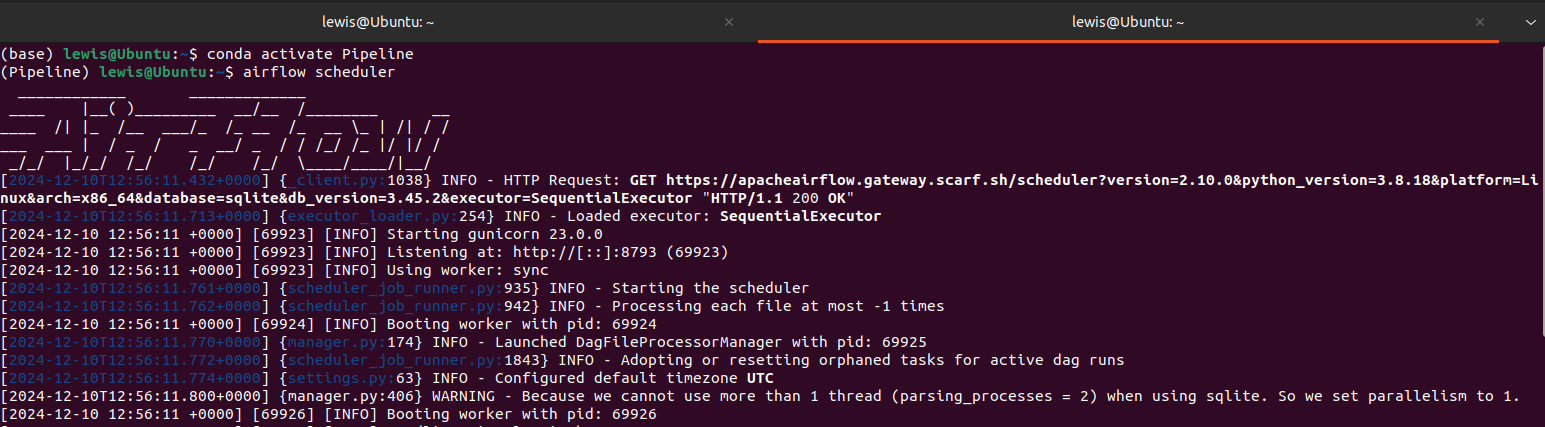
\includegraphics[width=\linewidth]{Implementation/Docker/Installation/5.png}
    \caption{Installing Docker.}
    \label{fig:DockerInstall5}
\end{figure}

\begin{figure}[H]
    \centering
    \includegraphics[width=\linewidth]{Implementation/Docker/Installation/6.png}
    \caption{Confirming that the Docker service is running.}
    \label{fig:DockerInstall6}
\end{figure}

\begin{figure}[H]
    \centering
    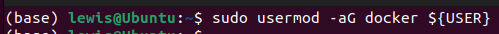
\includegraphics[width=\linewidth]{Implementation/Docker/Installation/7.png}
    \caption{Adding the VM user to the Docker group so they can execute commands.}
    \label{fig:DockerInstall7}
\end{figure}

\endgroup